\chapter[Modèle de Riesz]{Étude théorique du modèle de Riesz} % signal monogénique ?
\label{chap:chapitre1}

{\color{red} TODO : utiliser \\paragraph where needed}

Dans le but de synthétiser du contenu avec de la structure irrégulière, nous cherchons à avoir une approche locale. Pour cela nous utilisons le modèle du signal monogène~\cite{felsberg_monogenic_2001}, qui permet d'extraire l'énergie locale, en s'appuyant sur la transformée de Riesz. Ce SY procédé est ensuite mis en application dans un cadre multi-résolutionnel, en utilisant une pyramide de Riesz~\cite{wadhwa_riesz_2014} pour calculer la congruence de phases.

\section{Signal monogène}

Le signal monogène est un outil du domaine du traitement du signal, généralement utilisé pour des tâches d'analyse d'image ou de vision par ordinateur, comme la détection de caractéristiques. La revue de la méthode par Bridge~\cite{bridge_introduction_2018} est une bonne introduction aux principes théoriques du signal monogène ; nous reprennons dans cette partie sa notation et son discours exposé dans son document afin de prodiguer une compréhension du modèle.

\subsection{Une dimension, signal analytique}

\subsubsection{Construction du singal analytique}

Pour comprendre l'utilité du signal monogène, commençons par expliquer le fonctionnement du signal analytique, dont le signal monogène est l'extension aux signaux de dimension arbitraire. Le signal analytique est une méthode de représentation d'un signal 1D à valeurs réelles, qui facilite la manipulation et l'extraction de certaines informations du signal original. Le constat qui donne lieu à cette représentation est que pour un signal à valeurs réelles, les fréquences négatives sont superflues pour sa représentation de Fourier. En effet, on rappelle que la transformée de Fourier $F(\omega)$ d'un signal à valeurs réelles $f(t)$ présente une symétrie hermitienne :

\begin{equation}
    F(-\omega) = \overline{F(\omega)}
\end{equation}

avec $\overline{\cdot}$ l'opérateur de conjugaison complexe. L'idée est donc de se débarrasser des fréquences négatives, sans perte d'information, et de construire un nouveau signal en n'utilisant que les fréquences positives de $f(t)$. On exprime d'abord le signal $F_{\alpha}$ dans le domaine de Fourier :

\begin{equation}
    F_{\alpha}(\omega) = \left\{
    \begin{array}{ll}
        2F(\omega), & \omega > 0 \\
        0, & \omega < 0 \\
        F(0), & \omega = 0,
    \end{array}
    \right.
\end{equation}

où l'amplitude des composantes de fréquences positives est doublée, par soucis de conservation d'énergie. Avec cette formulation, toute l'information de notre signal original est conservée, mais cette nouvelle forme permet de faire des manipulations précédemment impossibles qui nous permettent de mieux comprendre notre signal.

\begin{figure}[h]
    %\noindent
    \hspace{-12pt}
    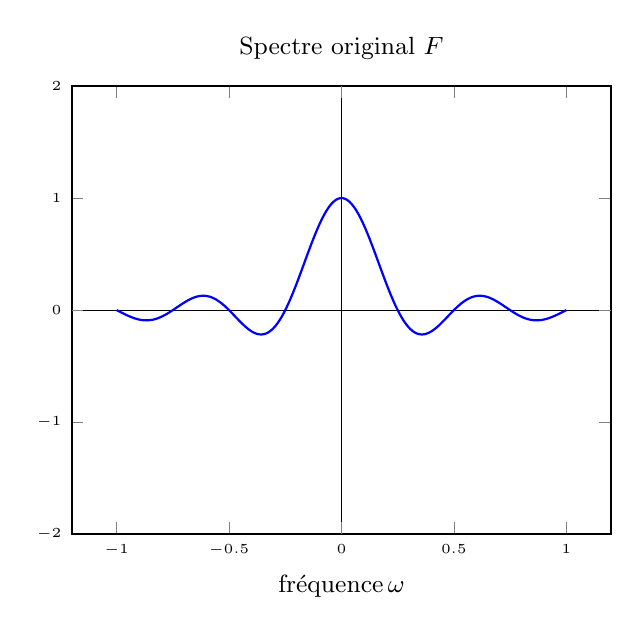
\begin{tikzpicture}
    \begin{axis}[
        title={Spectre original $F$},
        title style={font=\small},
        axis lines=box,
        style=thick,
        xlabel=\(\textnormal{fréquence}\, \omega\),
        xtick={-1, -0.5, 0.5, 1},
        ytick={-2, -1, 1, 2},
        extra x ticks=0,
        extra y ticks=0,
        extra x tick style={grid=major, grid style={black}},
        extra y tick style={grid=major, grid style={black}},
        tick label style={font=\tiny},
        label style={font=\small},
        ymin=-2, 
        ymax=2,
        ]
    \addplot[
        color=blue,
        domain=-1:1,
        samples=200
        ]
    {sin(360*x*2)/ (2*pi*x*2)};
    \end{axis}
    \end{tikzpicture}
    %\hskip 6pt
    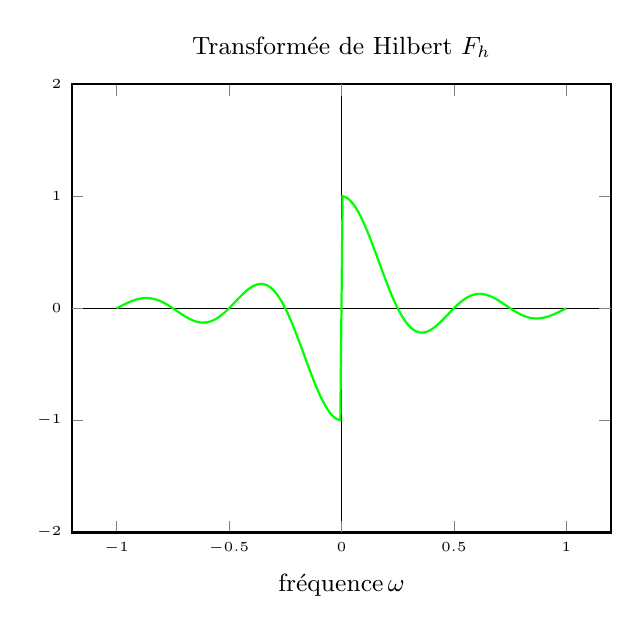
\begin{tikzpicture}
    \begin{axis}[
        title={Transformée de Hilbert $F_h$},
        title style={font=\small},
        axis lines=box,
        style=thick,
        xlabel=\(\textnormal{fréquence}\, \omega\),
        xtick={-1, -0.5, 0.5, 1},
        ytick={-2, -1, 1, 2},
        extra x ticks=0,
        extra y ticks=0,
        extra x tick style={grid=major, grid style={black}},
        extra y tick style={grid=major, grid style={black}},
        tick label style={font=\tiny},
        label style={font=\small},
        ymin=-2, 
        ymax=2,
        ]
    \addplot[
        color=green,
        domain=-1:1,
        samples=200
        ]
    {sign(x)*sin(360*x*2)/ (2*pi*x*2)};
    \end{axis}
    \end{tikzpicture}
    %\hskip 6pt
    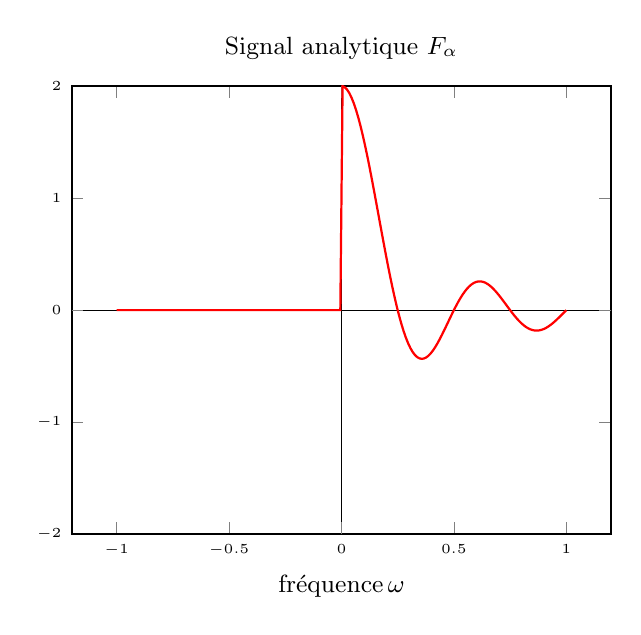
\begin{tikzpicture}
    \begin{axis}[
        title={Signal analytique $F_{\alpha}$},
        title style={font=\small},
        axis lines=box,
        style=thick,
        xlabel=\(\textnormal{fréquence}\, \omega\),
        xtick={-1, -0.5, 0.5, 1},
        ytick={-2, -1, 1, 2},
        extra x ticks=0,
        extra y ticks=0,
        extra x tick style={grid=major, grid style={black}},
        extra y tick style={grid=major, grid style={black}},
        tick label style={font=\tiny},
        label style={font=\small},
        ymin=-2, 
        ymax=2,
        ]
    \addplot[
        color=red,
        domain=-1:1,
        samples=200
        ]
    {(1+sign(x))*sin(360*x*2)/ (2*pi*x*2)};
    \end{axis}
    \end{tikzpicture}

    \caption[Signal analytique pour un signal simple]{Création du signal analytique dans le domaine fréquentiel (seule la partie réelle est montrée). Le signal original réel (gauche), qui présente une symétrie hermitienne, est ajouté à sa transformée de Hilbert (milieu), lui impair, pour former le signal analytique (droite), dépourvu de fréquence négative.}
    \label{fig:complex-analytic-representation}
\end{figure}

En effet, on peut voir le fait de supprimer les composantes de fréquences négatives comme le l'ajout d'un signal impair soigneusement choisi au signal de base.

\begin{equation} \label{eq:2.1}
    F_{\alpha}(\omega) = F(\omega) + F_h(\omega),
\end{equation}

où $F_h(\omega)$ est la « version impaire » du signal $F(\omega)$ :

\begin{equation}
    F_h(\omega) = \left\{
    \begin{array}{ll}
        F(\omega), & \omega > 0 \\
        -F(\omega), & \omega < 0 \\
        0, & \omega = 0,
    \end{array}
    \right.
\end{equation}

que l'on peut reformuler à l'aide de la fonction signe :

\begin{equation}
    F_h(\omega) = \sgn(\omega)\cdot F(\omega).
    \label{eq:2.5}
\end{equation}

On rappelle l'expression de la fonction signe :

\begin{equation}
    \sgn(x) = \left\{
    \begin{array}{ll}
        1, & x > 0 \\
        -1, & x < 0 \\
        0, & x = 0.
    \end{array}
    \right.
\end{equation}

On obtient alors la ré-écriture de l'équation~\ref{eq:2.1} :

\begin{equation}
    F_{\alpha}(\omega) = (1+\sgn(\omega))F(\omega)
\end{equation}

\begin{figure}[h]
    %\noindent
    %\hspace{-10pt}
    \centering
    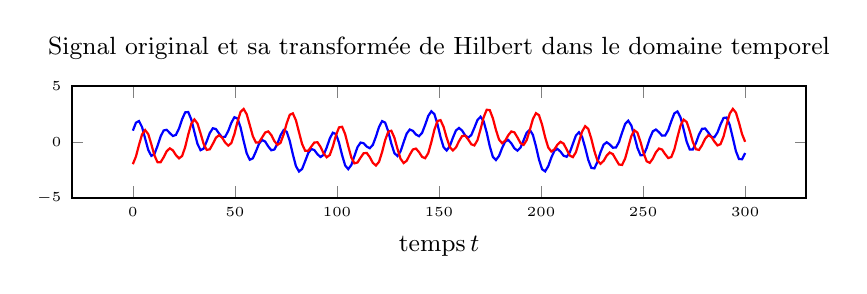
\begin{tikzpicture}
    \begin{axis}[
        title={Signal original et sa transformée de Hilbert dans le domaine temporel},
        title style={font=\small},
        axis lines=box,
        width=0.9\textwidth,
        height=3cm,
        style=thick,
        xlabel=\(\textnormal{temps}\, t\),
        xtick={0, 50, 100, 150, 200, 250, 300},
        ytick={-5, 0, 5},
        tick label style={font=\tiny},
        label style={font=\small},
        ymin=-5, 
        ymax=5,
        ]
    \addplot[
        color=blue,
        domain=0:300,
        samples=200
        ]
    {sin(3*x)+cos(15*x)+sin(30*x)};
    \addplot[
        color=red,
        domain=0:300,
        samples=200
        ]
    {-cos(3*x)+sin(15*x)-cos(30*x)};
    \end{axis}
    \end{tikzpicture}

    \caption[Signal analytique pour un signal complexe]{Exemple de représentation analytique. Le signal original réel (en bleu), et sa transformée de Hilbert imaginaire pure (en rouge).}
    \label{fig:analytic-representation}
\end{figure}


Le signal $F_{\alpha}$ créé est donc dans le domaine fréquentiel de $F$, signal original pair, de représentation purement réelle dans le domaine temporel, et de $F_h$, signal impair, de représentation purement imaginaire dans le domaine temporel, que l'on nomme $f_h$. Dans le domaine temporel, $f_{\alpha}$ est donc un signal complexe, sans composantes de fréquences négatives, c'est un signal analytique, que l'on appelle la \textit{représentation analytique} de $f$ :

\begin{equation}
    f_{\alpha}(t) = \underbrace{f(t)}_\text{réel pur} + \underbrace{f_h(t)}_\text{imaginaire pur}.
\end{equation}

Le signal ajouté pour annuler les fréquences $F_h$ est par ailleurs un objet connu : c'est la \textit{transformée de Hilbert} de $F$. Sa représentation, bien que très simple dans le domaine fréquentiel, est difficile à obtenir et manipuler dans le domaine temporel :

\begin{equation}
    f_h(t) = i \cdot \textnormal{p.v.} \int_{-\infty}^{\infty} \frac{f(t)}{\pi(t-\tau)} \,d\tau,
\end{equation}

où p.v. est la valeur principale de Cauchy, nécessaire pour cette intégrale, qui représente la convolution avec la distribution $\frac 1{\pi t}$ et qui est impropre à cause de la singularité en $t=\tau$. Cependant, dû à la complexité de cet objet, nous utiliserons majoritairement l'expression fréquentielle de la transformée de Hilbert :

\begin{align*}
    &\hil(F) = F_h = \sgn\cdot F \\
    &\mathcal{H}(F) = F_h = \sgn\cdot F
\end{align*}


\subsubsection{Amplitude et phase locales}

Pour comprendre l'intérêt du signal analytique, on étudie d'abord l'exemple d'une fonction sinusoïdale, d'amplitude $A$ et de fréquence $\omega_0$ fixées :

\begin{equation}
    f(t) = A\sin(\omega_0t).
\end{equation}

En utilisant les relations montrées précédemment, on trouve la transformée de Hilbert de $f$ et on calcule sa représentation analytique :

\begin{align}
    f_h(t) &= iA\cos(\omega_0t) \\
    f_{\alpha}(t) &= f(t) + f_h(t) \\
    &= A\sin(\omega_0t)+iA\cos(\omega_0t) \\
    &= Ae^{i\omega_0t}.
\end{align}

Pour une sinusoïde, la transformée de Hilbert est un simple \textit{déphasage} de $-\frac{\pi}2$ du signal original. Or la théorie de Fourier nous indique que n'importe quel signal générique peut être décomposé comme une somme de sinusoïdes. Ainsi la transformée de Hilbert agit de la même manière sur tous les signaux : c'est un déphasage de $-\frac{\pi}2$ de chaque composante fréquentielle qui compose le signal. Le signal $f$ et sa transformée de Hilbert $f_h$ sont dit en \textit{quadrature de phase}, et le signal analytique s'exprime comme une exponentielle complexe.

\bigskip

En fait, puisque tout signal est maintenant représenté comme la somme d'un réel et d'un imaginaire pur, on peut toujours l'exprimer en coordonnées polaires comme une exponentielle complexe, d'amplitude et phase variant au cours du temps :

\begin{equation}
    f_{\alpha} (t) = A(t)e^{i\phi(t)}.
\end{equation}

avec 

\begin{align}
    A(t) &= \sqrt{f(t)^2 + h_h(t)^2} \\
    \phi(t) &= \arctan\left(\frac{f_h(t)}{f(t)}\right).
\end{align}

Cette représentation introduit le concept d'\textit{amplitude locale} et de \textit{phase locale} (ici \textit{temporellement} locales), qui sont deux outils d'analyse particulièrement intéressants pour l'étude approfondie du signal original. L'amplitude locale agit comme une mesure de l'\textit{enveloppe} du signal, et la phase locale comme une mesure de la \textit{forme} du signal. Par exemple, une phase de $0$ indique un extremum, et une phase de $\pm\pi$ indique un passage par zéro. La figure~\ref{fig:local-pha-amp} montre un signal avec son amplitude locale et sa phase locale. À partir uniquement de notre signal initial, on a ainsi créé un outil nous permettant d'obtenir de l'information bien plus intéressante sur l'apparence et les propriétés du signal.

\begin{figure}[h]

    \centering
    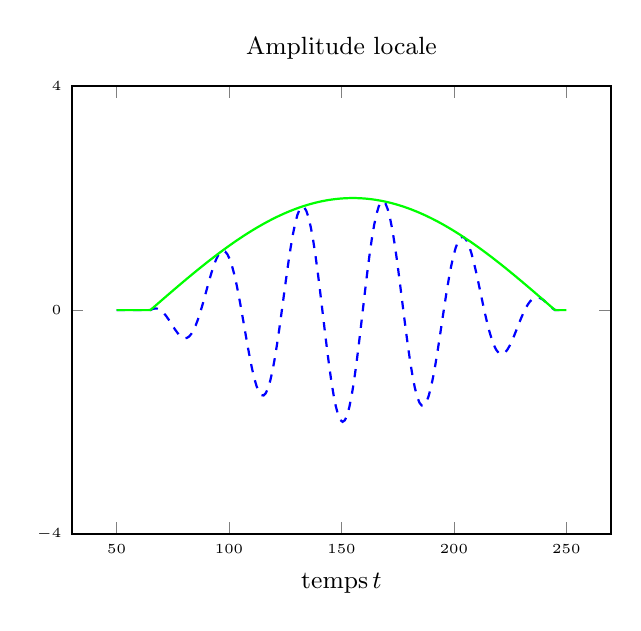
\begin{tikzpicture}
    \begin{axis}[
        title={Amplitude locale},
        title style={font=\small},
        axis lines=box,
        %width=0.9\textwidth,
        %height=3cm,
        style=thick,
        xlabel=\(\textnormal{temps}\, t\),
        xtick={50, 100, 150, 200, 250},
        ytick={-4, 0, 4},
        tick label style={font=\tiny},
        label style={font=\small},
        ymin=-4, 
        ymax=4,
        ]
    \addplot[
        color=blue,
        domain=50:250,
        samples=200,
        style=dashed,
        ]
    {(sign(x-65)-sign(x-245))*sin(10*x+25)*cos(x+25)};
    \addplot[
        color=green,
        domain=50:250,
        samples=200
        ]
    {(sign(x-65)-sign(x-245))*sqrt((0.5*(sin(11*x-40) + sin(9*x-90)))^2 + (sin(10*x+25)*cos(x+25))^2)};
    \end{axis}
    \end{tikzpicture}
    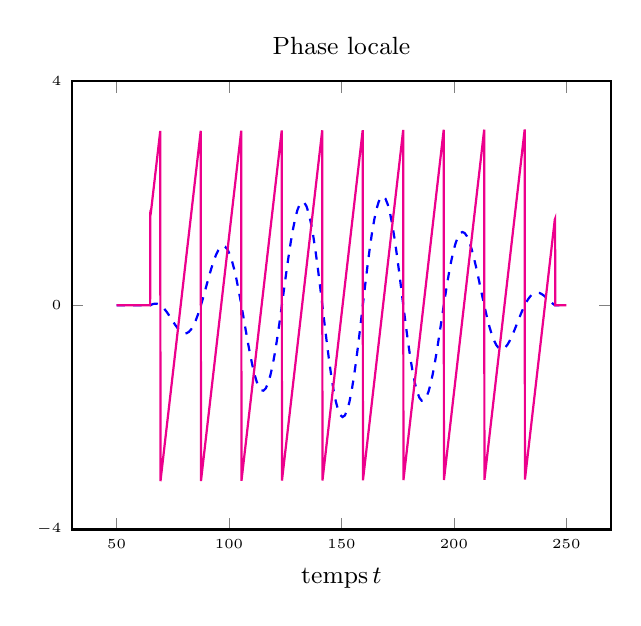
\begin{tikzpicture}
    \begin{axis}[
        title={Phase locale},
        title style={font=\small},
        axis lines=box,
        %width=0.9\textwidth,
        %height=3cm,
        style=thick,
        xlabel=\(\textnormal{temps}\, t\),
        xtick={50, 100, 150, 200, 250},
        ytick={-4, 0, 4},
        tick label style={font=\tiny},
        label style={font=\small},
        ymin=-4, 
        ymax=4,
        ]
    \addplot[
        color=blue,
        domain=50:250,
        samples=200,
        style=dashed,
        ]
    {(sign(x-65)-sign(x-245))*sin(10*x+25)*cos(x+25)};
    \addplot[
        color=magenta,
        domain=50:250,
        samples=2000
        ]
    {(sign(x-65)-sign(x-245))*rad(atan((0.5*(sin(11*x-40) + sin(9*x-90))) / (sin(10*x+25)*cos(x+25))))};
    \end{axis}
    \end{tikzpicture}

    \caption[Informations locales pour un signal simple]{Extraction d'informations locales pour un cosinus modulé par un sinus. L'amplitude locale (gauche) donne l'enveloppe de la sinusoïde, et la phase locale (droite) nous donne de l'information quant à la position dans le cycle d'oscillation.}
    \label{fig:local-pha-amp}

\end{figure}

\subsubsection{Notion d'échelle}
\label{subsubsec:echelle}

L'exemple donné avec la figure~\ref{fig:local-pha-amp} fonctionne bien car le signal est simple, l'interprétation de l'amplitude et la phase locale est claire et visuelle. Pour un signal plus complexe, plus représentatif des signaux que l'on doit souvent étudier, ce n'est pas si facile. La figure~\ref{fig:complex-local-pha-amp} affiche les informations locales du signal de la figure~\ref{fig:analytic-representation}, une somme de trois sinusoïdes de fréquences différentes ; il est moins évident de comprendre ce que les informations locales représentent dans ce cas.

\begin{figure}[h]
    \centering
    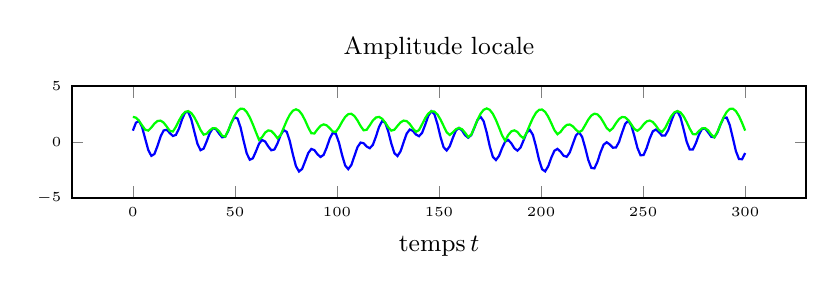
\begin{tikzpicture}
    \begin{axis}[
        title={Amplitude locale},
        title style={font=\small},
        axis lines=box,
        width=0.9\textwidth,
        height=3cm,
        style=thick,
        xlabel=\(\textnormal{temps}\, t\),
        xtick={0, 50, 100, 150, 200, 250, 300},
        ytick={-5, 0, 5},
        tick label style={font=\tiny},
        label style={font=\small},
        ymin=-5, 
        ymax=5,
        ]
    \addplot[
        color=blue,
        domain=0:300,
        samples=200
        ]
    {sin(3*x)+cos(15*x)+sin(30*x)};
    \addplot[
        color=green,
        domain=0:300,
        samples=200
        ]
    {sqrt((sin(3*x)+cos(15*x)+sin(30*x))^2 + (-cos(3*x)+sin(15*x)-cos(30*x))^2)};
    \end{axis}
    \end{tikzpicture}
    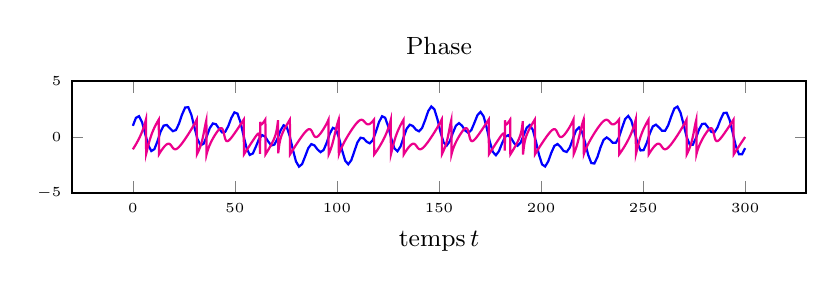
\begin{tikzpicture}
    \begin{axis}[
        title={Phase},
        title style={font=\small},
        axis lines=box,
        width=0.9\textwidth,
        height=3cm,
        style=thick,
        xlabel=\(\textnormal{temps}\, t\),
        xtick={0, 50, 100, 150, 200, 250, 300},
        ytick={-5, 0, 5},
        tick label style={font=\tiny},
        label style={font=\small},
        ymin=-5, 
        ymax=5,
        ]
    \addplot[
        color=blue,
        domain=0:300,
        samples=200
        ]
    {sin(3*x)+cos(15*x)+sin(30*x)};
    \addplot[
        color=magenta,
        domain=0:300,
        samples=3000
        ]
    {rad(atan((-cos(3*x)+sin(15*x)-cos(30*x)) / (sin(3*x)+cos(15*x)+sin(30*x))))};
    \end{axis}
    \end{tikzpicture}    

    \caption[Informations locales pour un signal complexe]{Informations locales pour un signal complexe, somme de plusieurs sinusoïdes. Pour un tel signal, l'interprétation des informations locales est moins évidente.}
    \label{fig:complex-local-pha-amp}
\end{figure}

Le problème à l'analyse de ce signal est le fait qu'il existe plusieurs niveaux de structure, qui interfèrent et rendent l'interprétation des informations locales impossible à l'échelle macroscopique.
Pour extraire de l'information utile, il faut sélectionner et faire l'analyse d'un seul niveau de structure, donc d'échelle.
Pour cela, on filtre les composantes des niveaux qui ne nous intéressent pas.
Pour se faire, il est possible d'utiliser des filtres passe-bande, comme le fait Bridge avec les filtres log-Gabor, un choix commun pour ce genre de pratique.
Un filtre log-Gabor est un filtre défini dans le domaine fréquentiel, qui permet de sélectionner une bande de fréquence centrée autour d'une fréquence centrale $\omega_0$.
Il a une réponse en fréquence de forme gaussienne quand observé en échelle logarithmique :

\begin{equation}
    G(\omega) = \exp\left(-\frac{\log^2(\frac{|\omega|}{\omega_0})}{2\log(\sigma_0)^2}\right).
\end{equation}

Ces filtres sont caractérisés par deux paramètres : la fréquence centrale $\omega_0$, qui contrôle quelle échelle de structure est sélectionnée, et la largeur de bande $\sigma_0$, un paramètre de forme qui contrôle la largeur de la bande de fréquence sélectionnée. Des exemples de filtre log-Gabor sont montrés à la figure~\ref{fig:log-gabor-filters}.

En appliquant un filtre log-Gabor à notre signal avant de lui appliquer la transformée de Hilbert et de déterminer sa représentation analytique, on obtient une représentation locale du signal, centrée autour d'une fréquence $\omega_0$ et d'une échelle $\sigma_0$ que l'on peut faire varier arbitrairement.

\begin{equation}
    F_{\alpha}(\omega) = (1+\sgn(\omega))G(\omega)F(\omega)
\end{equation}

\begin{figure}
    \centering
    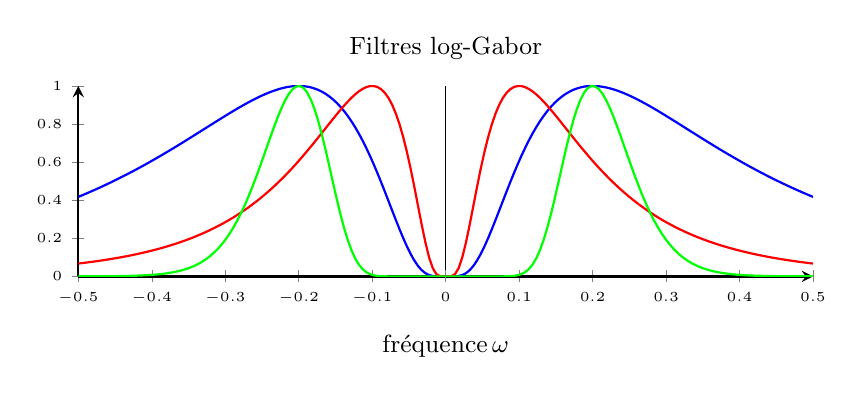
\begin{tikzpicture}
    \begin{axis}[
        title={Filtres log-Gabor},
        title style={font=\small},
        axis lines=left,
        width=0.9\textwidth,
        height=4cm,
        style=thick,
        xlabel=\(\textnormal{fréquence}\, \omega\),
        xtick={-0.5, -0.4, -0.3, -0.2, -0.1, 0.1, 0.2, 0.3, 0.4, 0.5},
        ytick={0, 0.2, 0.4, 0.6, 0.8, 1},
        tick label style={font=\tiny},
        label style={font=\small},
        extra x ticks=0,
        extra x tick style={grid=major, grid style={black}},
        ymin=0,
        ymax=1,
        ]
    \addplot[
        color=blue,
        domain=-0.5:0.5,
        samples=200
        ]
    {exp(-ln(abs(x)/.2)^2 / (2*ln(.5)^2))};
    \addplot[
        color=red,
        domain=-0.5:0.5,
        samples=200
        ]
    {exp(-ln(abs(x)/.1)^2 / (2*ln(.5)^2))};
    \addplot[
        color=green,
        domain=-0.5:0.5,
        samples=200
        ]
    {exp(-ln(abs(x)/.2)^2 / (2*ln(.8)^2))};
    \end{axis}
    \end{tikzpicture}

    \caption[Filtres log-Gabor]{Représentation dans le domaine fréquentiel de filtres log-Gabor de différents paramètres. En rouge, $\omega_0=0.1, \sigma_0 = 0.5$. En bleu, $\omega_0=0.2, \sigma_0 = 0.5$. En vert, $\omega_0=0.2, \sigma_0 = 0.8$.}
    \label{fig:log-gabor-filters}
\end{figure}

En étudiant la réponse du signal sur une large gamme de fréquences et d'échelles, on obtient une représentation locale du signal à différentes échelles, et ainsi extraire de l'information sur les différentes structures du signal. On peut rassembler toutes ces informations dans un graphique appelé scalogramme, qui représente le comportement de la phase locale en fonction du temps et de l'échelle, comme montré à la figure~\ref{fig:scalogram}. On y voit facilement les différents niveaux de structure du signal, et l'interprétation des informations locales devient plus utile car on peut choisir à quel niveau on regarde.

Si l'on compare le modèle du signal analytique à celui de la transformée de Fourier, on remarque que les informations que l'on obtient avec les deux diffèrent et se complètent. La transformée de Fourier nous donne de l'information globale sur tout le signal, mais localisée en termes de fréquence. La représentation analytique, elle, nous donne une information spatialement locale sur le signal, mais sur une bande de fréquences, sélectionnées par un filtre passe-bande. Le modèle d'information locale est donc un compromis entre la localisation spatiale et fréquentielle, et permet d'obtenir une information différente sur le signal.


\begin{figure}
    \centering
    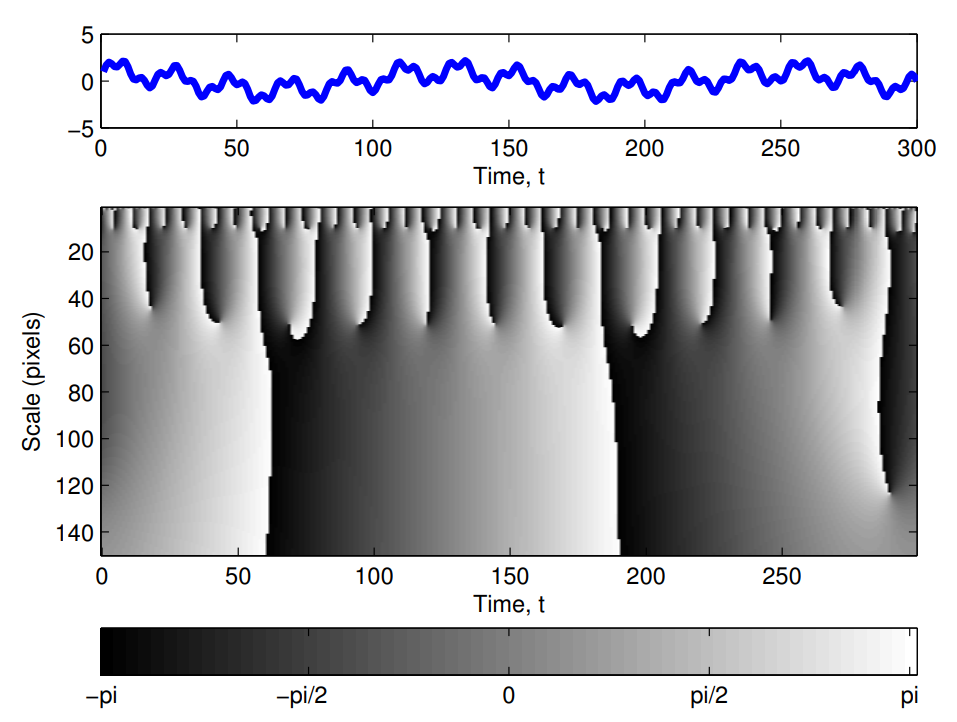
\includegraphics[width=\textwidth]{contenu/resources/images/scalogram}
    \caption[Scalogramme de la phase locale]{Scalogramme de la phase locale pour un signal complexe. La phase locale est représentée en échelle de gris, et varie en fonction du temps (en abscisse) et de l'échelle en nombre de pixels (en ordonnée). Diagramme par Bridge~\cite{bridge_introduction_2018}.}
    \label{fig:scalogram}
\end{figure}


\subsection{Deux dimensions, signal monogène}

Le modèle du signal analytique est utile à l'extraction d'informations locales pour des signaux 1D, et il serait intéressant d'avoir accès à ces informations pour des images, donc des signaux 2D. En effet l'importance de la phase dans l'analyse d'image a déjà été soulignée depuis longtemps~\cite{oppenheim_importance_1981}. Cependant, l'application n'est pas directe dans le cas de deux (ou plus) dimensions, car il y a une notion de direction à considérer. C'est ce que le modèle du signal monogène, proposé par Felsberg et Sommer~\cite{felsberg_monogenic_2001}, permet de faire, et que nous allons développer dans cette partie.

\subsubsection{Construction du signal monogène}

Pour créer la représentation analytique d'un signal 1D, on SY génère un imaginaire pur, en quadrature de phase avec le signal original, en utilisant la transformée de Hilbert. Pour un signal 2D, on a besoin de former deux « parties imaginaires », une pour chaque direction. On ne peut donc pas représenter le signal monogène comme un complexe. Pour un traitement exact, il faudrait utiliser les quaternions, que l'on peut voir comme une extension des nombres complexes à une plus haute dimension. Pour simplifier la compréhension et manipulation, on peut cependant se passer de la théorie des quaternions, et traiter le signal monogène comme s'il avait trois parties réelles distinctes dans un premier temps.
Pour générer les parties impaires du signal, on utilise une généralisation de la transformée de Hilbert à plusieurs dimensions, la \textit{transformée de Riesz}. Soit $f$ un signal d'un espace 2D de la variable $\mathbf{x} = (x, y)^T$, et $F$ sa représentation dans le domaine fréquentiel obtenue par transformée de Fourier 2D, avec $\mathbf{\omega}=(\omega_x, \omega_y)^T$ une fréquence 2D. Alors les parties impaires de $f$, $F_{o1}$ et $F_{o2}$, sont données par :

\begin{align}
    F_{o1}(\mathbf{\omega}) &= \widehat{\mathcal{R}_1(f)}(\mathbf{\omega}) =
        \left\{
        \begin{array}{ll}
            -i\frac{\omega_x}{||\omega||}F(\omega), & \omega > 0 \\
            0, & \omega = 0,
        \end{array}
        \right. \\
    F_{o2}(\mathbf{\omega}) &= \widehat{\mathcal{R}_2(f)}(\mathbf{\omega}) =
        \left\{
        \begin{array}{ll}
            -i\frac{\omega_y}{||\omega||}F(\omega), & \omega > 0 \\
            0, & \omega = 0.
        \end{array}
        \right.
    \label{eq:2.20}
\end{align}

Avec cette définition de $F_{o1}$ et $F_{o2}$, on a que les signaux correspondant dans le domaine spatial sont des signaux à valeurs réelles. En effet un signal 2D à valeurs réelles $f$ a un spectre dont la partie réelle est paire, et la partie imaginaire impaire, soit :

\begin{equation}
    Re\{F(\omega)\} = Re\{F(-\omega)\}, \quad Im\{F(\omega)\} = -Im\{F(-\omega)\}.
\end{equation}

Dans la définition~\ref{eq:2.20}, comme $F$ est le spectre d'un signal réel, on a que $F_{o1}$ et $F_{o2}$ vérifient ces propriétés de symétrie, et donc que les signaux correspondants dans le domaine spatial sont bien réels.

Si l'on compare à comment la transformée de Hilbert est formée~\ref{eq:2.5}, on remarque que ces parties impaires sont des versions généralisées de la transformée de Hilbert, où l'on prend en compte la direction de la fréquence. Chaque composante fréquentielle dans ces parties impaires est déphasée de $-\pi/2$ et mise à l'échelle de telle sorte que l'amplitude soit partagée entre les deux parties.

\begin{figure}
    \centering
    \begin{subfigure}[b]{.3\textwidth}
        
\includegraphics[width=\textwidth]{contenu/resources/images/disk}
        \caption{Signal original}
    \end{subfigure}
    \hfill
    \begin{subfigure}[b]{.3\textwidth}
        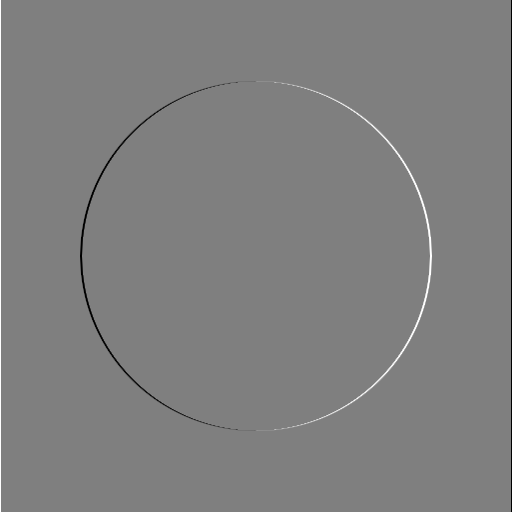
\includegraphics[width=\textwidth]{contenu/resources/images/r2_disk}
        \caption{Première partie impaire}
    \end{subfigure}
    \hfill
    \begin{subfigure}[b]{.3\textwidth}
        
\includegraphics[width=\textwidth]{contenu/resources/images/r1_disk}
        \caption{Seconde partie impaire}
    \end{subfigure}
    \caption[Visualisation du signal monogène pour un disque]{Visualisation du signal monogène pour un disque : le signal original $f$ (gauche), et ses parties impaires $f_{o1}$ (milieu) et  $f_{o2}$ (droite), affichées avec une échelle de couleurs encodant la valeur, de -1 (noir) à +1 (blanc).}
    \label{fig:monogenic-signal-disk}
\end{figure}

On obtient ainsi une expression du signal monogène comme un vecteur à trois composantes, une paire et deux impaires :

\begin{equation}
    f_m(\mathbf{x}) =
    \left[
        \begin{array}{c}
        f_e(\mathbf{x}) \\
        f_{o1}(\mathbf{x}) \\
        f_{o2}(\mathbf{x})
        \end{array}
    \right],
\end{equation}

où $f_e$ est le signal original, indexé par un $e$ pour souligner qu'il représente la partie paire du signal monogène. Une représentation d'un signal et de ses parties impaires est présentée à la figure~\ref{fig:monogenic-signal-disk}. On remarque notamment que les parties impaires détectent des changements verticaux et horizontaux dans le signal. Ceci est dû au fait que la transformée de Riesz présente une ressemblance et une connexion au gradient (l'équation~\ref{eq:2.20} rappelle fortement la définition du gradient, à un facteur près), que présente aussi d'ailleurs la transformée de Hilbert en une dimension. Ce rapport au gradient ne sera cependant pas exploré plus en profondeur dans la suite de ce travail.

Il est aussi commun de se représenter le signal monogène comme un vecteur de deux composantes seulement, une paire et une impaire, où cette dernière est en fait une combinaison des deux parties impaires présentées ici. Cette représentation est plus compacte, mais ce au détriment de la perte d'information sur l'orientation. Elle sera parfois utilisée dans la suite de ce travail :

\begin{equation}
    f_o(\mathbf{x}) = \sqrt{f_{o1}(\mathbf{x})^2 + f_{o2}(\mathbf{x})^2}.
\end{equation}

La transformée de Riesz peut s'exprimer directement dans le domaine spatial, mais comme la transformée de Hilbert, elle n'est représentable que par un objet mathématique compliqué, une intégrale singulière :

\begin{equation}
    R_if(x) = c_d \lim_{\epsilon \to 0}\int_{\mathbb{R}^d\setminus B_\epsilon(x)}\frac{(x_i-t_i)f(t)}{|x-t|^{d+1}}\,dt,
    \label{eq:riesz-transform-spatial}
\end{equation}

pour $i\in\llbracket 0, d\rrbracket$ avec $d$ la dimension, et où $c_d$ est une constante de normalisation dimensionnelle :

\begin{equation}
    c_d = \frac1{\pi\omega_{d-1}} = \frac{\Gamma((d+1)/2)}{\pi^{(d+1)/2}},
\end{equation}

avec $\omega_{d-1}$ le volume de la $(d-1)$-sphère unité. Au vue de la complexité de calcul et de manipulation de cette expression, nous utiliserons plutôt la formulation fréquentielle dans la suite du travail.

\subsubsection{Amplitude, phase et orientation locales}

Avec cet outil qu'est le signal monogène, on peut maintenant étendre les concepts d'informations locales à nos images, qui sont des signaux 2D. En 1D, on a deux parties pour le signal analytique, que l'on représente en coordonnées polaires avec l'amplitude et la phase. En 2D, on a trois coordonnées, que l'on représente donc en coordonnées sphériques où sont définis le rayon, l'angle d'élévation et l'azimut, comme montré en figure~\ref{fig:spherical-representation}.

\begin{figure}
    \centering
    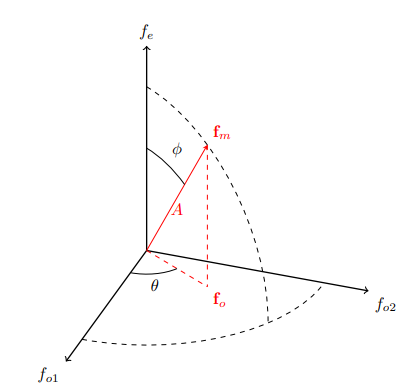
\includegraphics[width=.45\textwidth]{contenu/resources/images/spherical_representation}
    \caption[Représentation du signal monogène en coordonnées sphériques]{Représentation du signal monogène $f_m$ (rouge) en coordonnées sphériques, où les axes sont les différentes parties du signal. Le rayon représente l'amplitude locale, l'angle d'élévation $\phi$ la phase locale, et l'azimut $\theta$ l'orientation locale.}
    \label{fig:spherical-representation}
\end{figure}

L'amplitude locale $A$ représente, comme en 1D, le rayon de la représentation :

\begin{align}
    A(\mathbf{x}) &= \sqrt{f_e(\mathbf{x})^2 + f_{o1}(\mathbf{x})^2 + f_{o2}(\mathbf{x})^2} \\
    &= \sqrt{f_e(\mathbf{x})^2 + f_o(\mathbf{x})^2}.
\end{align}

La phase locale $\phi$ mesure l'angle entre la partie paire $f_e$ et la partie impaire combinée $f_o$, et représente donc l'angle d'élévation de la représentation :

\begin{equation}
    \phi(\mathbf{x}) = \arctan\left(\frac{f_o(\mathbf{x})}{f_e(\mathbf{x})}\right).
\end{equation}

Enfin l'orientation locale $\theta$ complète la représentation en donnant l'angle d'azimut, soit la direction dominante dans l'image à cet endroit, exprimé comme l'orientation de la partie impaire $f_o$ :

\begin{equation}
    \theta(\mathbf{x}) = \arctan\left(\frac{f_{o2}(\mathbf{x})}{f_{o1}(\mathbf{x})}\right).
\end{equation}

La figure~\ref{fig:monogenic-local-representation} montre un exemple de représentation locale pour une image, avec l'amplitude, la phase et l'orientation locales.

\begin{figure}
    \centering
    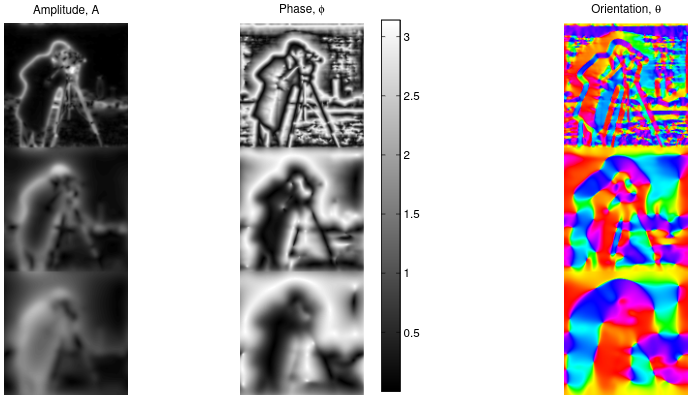
\includegraphics[width=\textwidth]{contenu/resources/images/local_information_monogenic}
    \caption[Représentation locale du signal monogène]{Représentation locale du signal monogène pour une image, avec l'amplitude (gauche), la phase (milieu) et l'orientation (droite) locales. Image par Bridge~\ref{bridge_introduction_2018}.}
    \label{fig:monogenic-local-representation}
\end{figure}

Le changement de représentation est réversible, et on peut retrouver le signal monogène à partir des informations locales :

\begin{equation}
    f_m(\mathbf{x}) = A(\mathbf{x})\left[
        \begin{array}{c}
        \cos(\phi(\mathbf{x})) \\
        \sin(\phi(\mathbf{x}))\cos(\theta(\mathbf{x})) \\
        \sin(\phi(\mathbf{x}))\sin(\theta(\mathbf{x}))
        \end{array}
    \right].
\end{equation}

L'image originale notamment s'exprime simplement par $f(\mathbf{x}) = A(\mathbf{x})\cos(\phi(\mathbf{x}))$. Nous utiliserons cette formule plus tard dans nos travaux pour reconstruire nos images après avoir modifié leurs informations locales.

\bigskip

Comme pour le signal analytique en 1D, il est intéressant d'utiliser des filtres pour sélectionner un niveau d'échelle à analyser, afin d'extraire de l'information sur certains niveaux de structure en particulier. Ici encore, on peut utiliser des filtres log-Gabor pour séléctionner les parties du signal qui nous intéressent.

\begin{figure}
    \centering
    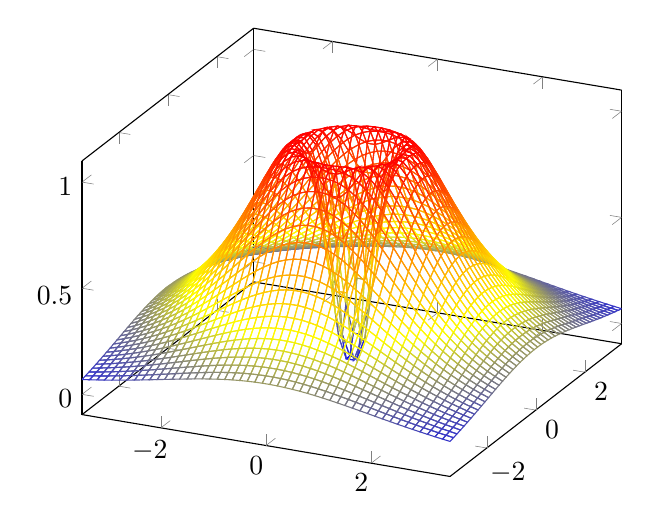
\begin{tikzpicture}
    \begin{axis}[
        colormap/hot,
%        xtick={-.5, 0, .5},
%        ytick={-.5, 0, .5},
%        ztick={-1, 0, 1}
    ]
        \addplot3[
        mesh,
        samples=50,
        domain=-3.5:3.5,
        ]
        {exp(-(ln(sqrt(x^2+y^2))^2)/(2*ln(.5)^2))};
    \end{axis}
    \end{tikzpicture}

    \caption[Filtre log-Gabor en 2D]{Représentation en domaine fréquentiel d'un filtre log-Gabor. Comme en 1D, le filtre sélectionne une bande de fréquence centrée autour d'une fréquence centrale $\omega_0$, et de largeur de bande $\sigma_0$.}
    \label{fig:2D-log-gabor}
\end{figure}

Avec ces filtres, on calcule les parties paires et impaires du signal en sélectionnant plusieurs échelles différentes, et on obtient ainsi une représentation locale qui met en valeur différents niveaux de structure présents dans l'image. La figure~\ref{fig:cameraman-monogenic} montre une image et son signal monogénique, calculé sur plusieurs niveaux d'échelle.

\begin{figure}
    \centering
    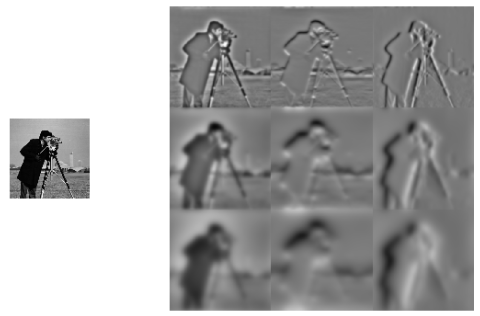
\includegraphics[width=.75\textwidth]{resources/images/cameraman_monogenic}
    \caption[Signal monogène calculé pour plusieurs niveaux d'échelle]{Image originale (gauche) et son signal monogène (droite), calculé sur plusieurs niveaux d'échelle. Dans l'image de droite : en colonne les différentes parties, paire $f_e$ (gauche), impaire 1 $f_{o1}$ (milieu) et impaire 2 $f_{o2}$ (droite). En ligne les longueurs d'onde centrale $\lambda_0 = 2\pi/\omega_0$, caractéristiques de l'échelle de structure détectée : $\lambda_0 = 20$~pixels (haut), $\lambda_0 = 60$~pixels (milieu), $\lambda_0 = 100$~pixels (bas). Pour référence, la taille de l'image originale est 256 $\times$ 256 pixels. Image par Bridge~\cite{bridge_introduction_2018}.}
    \label{fig:cameraman-monogenic}
\end{figure}



\bigskip
{#color{red} SY cadre de travail}
Maintenant que notre cadre de travail pour le restant du manuscript, le signal monogène, a été plus formellement introduit, nous allons pouvoir nous intéresser RE au cadre que nous avons choisi pour travailler à différents niveaux de structure. Bridge présente dans son article~\cite{bridge_introduction_2018} un cadre de travail utilisant les filtres log-Gabor, qui possèdent une expression complexe dans le domaine temporel. Pour nos travaux, nous avons utilisé une autre méthode de représentation, la pyramide de Riesz, plus simple à calculer et manipuler, et qui nous permet de nous concentrer sur l'analyse de textures. Nous allons maintenant présenter cette pyramide de Riesz, et montrer comment elle peut être utilisée pour l'analyse de textures.

\section{Pyramide de Riesz}

% Pyramide d'image inventée par Burt et Adelson~\cite{burt_laplacian_1983} pour la compression d'image.
L'idée d'utiliser une pyramide d'image est introduite par Simoncelli et al.~\cite{simoncelli_shiftable_1992}, {\color{red}REFOLMURER dans le but d'avoir une représentation possédant des bonnes propriétés d'études.}. C'est une méthode de représentation multi-échelle d'une image.
% AVANTAGES de la pyramide d'image de Simoncelli, la complex steerable pyramid :
% - steerable, invariance par rotation
% - invariance par translation et mise à l'échelle
% - avoids spatial aliasing
SY Conceptuellement, une pyramide d'image remplit la même fonction qu'une banque de filtres, comme les filtres log-Gabor utlisés par Bridge : on décompose une image en s'intéressant successivement à différentes bandes de fréquences, afin d'extraire de l'information localisée en fréquence. La pyramide que nous utilisons, inspirée de Wadhwa et al.~\cite{wadhwa_phase_based_2013}, est construite en formant dans un premier temps la pyramide de Gauss, puis de Laplace de l'image, qui elle nous sert à avoir une méthode de reconstruction de notre image. On applique ensuite la transformée de Riesz à tous les étages de la pyramide, pour obtenir le signal monogène de chaque niveau. De là, on extrait les informations locales à tous les niveaux de structure, informations qui seront ultérieurement utilisées pour l'analyse et la synthèse de nos textures.

\subsection{Pyramide gaussienne}

RE La méthode de pyramide d'image est une méthode de représentation multi-échelle d'une image, répandue dans les domaines de la vision par ordinateur et du traitement d'image. Initialement introduite par Burt et Adelson~\cite{burt_laplacian_1983} pour la compression d'image, elle permet d'étudier une image à différents niveaux de résolution, afin de faciliter la détection de motifs en sélectionnant le niveau d'échelle correspondant au motif recherché. Elle est ensuite étendue par Simoncelli et al.~\cite{simoncelli_shiftable_1992} pour RE avoir une représentation possédant des bonnes propriétés d'études. 

Il existe deux types principaux de pyramide, passe-bas et passe-bande. Pour créer une pyramide passe-bas, aussi dite de Gauss, on procède itérativement suivant les deux étapes qui suivent :

\begin{itemize}
    \item une étape de \textit{lissage} (ou filtrage) de l'image, qui consiste à appliquer un filtre passe-bas à l'image, afin de supprimer les hautes fréquences. On obtient ainsi une image lissée, où les détails fins ont été supprimés ;
    \item une étape de \textit{sous-échantillonnage}, qui consiste à réduire la taille de l'image en gardant un pixel sur deux dans chaque direction. On obtient ainsi une image de moitié de la taille de l'image originale.
\end{itemize}

On répète ces deux étapes sur l'étage nouvellement créé, et ce jusqu'à atteindre la profondeur désirée. On se retrouve ainsi avec une collection d'images de plus en plus petites et de moins en moins raffinées (en termes de résolution), qui peut graphiquement être représentée comme une pyramide, en superposant les étages du plus grand au plus petit, comme montré à la figure~\ref{fig:gaussian-pyramid}.

\begin{figure}[h]
    \centering

    \begin{subfigure}{.3\textwidth}
        \centering
        
\includegraphics[width=\textwidth]{contenu/resources/images/gauss_0}
        \caption{Image originale}
    \end{subfigure}
    \hfill
    \begin{subfigure}{.3\textwidth}
        \centering
        
\includegraphics[width=\textwidth]{contenu/resources/images/gauss_3}
        \caption{Étage 3}
    \end{subfigure}
    \hfill
    \begin{subfigure}{.3\textwidth}
        \centering
        
\includegraphics[width=\textwidth]{contenu/resources/images/gauss_5}
        \caption{Étage 5}
    \end{subfigure}
%    \hfill
%    \begin{subfigure}{.22\textwidth}
%        \centering
%        
\includegraphics[width=\textwidth]{contenu/resources/images/gauss_3}
%        \caption{Étage 3}
%    \end{subfigure}

    \caption[Pyramide de Gauss]{Pyramide de Gauss. De gauche à droite, on descend dans les étages de plus en plus petits.}
    \label{fig:gaussian-pyramid}
\end{figure}

Plusieurs noyaux de lissage différents ont été proposés dans la littérature, comme la famille des noyaux binomiaux que nous utilisons dans notre implémentation RE en suivant l'exemple de la bibliothèque de traitement d'images OpenCV. Notre noyau de convolution s'exprime à l'aide des coefficients binomiaux :

\begin{equation}
    k = \frac{1}{256}\left[
        \begin{array}{ccccccc}
            1 & 4 & 6 & 4 & 1 \\
            4 & 16 & 24 & 16 & 4 \\
            6 & 24 & 36 & 24 & 6 \\
            4 & 16 & 24 & 16 & 4 \\
            1 & 4 & 6 & 4 & 1
        \end{array}
    \right],
\end{equation}

Il est intéressant de constater que les pyramides gaussiennes sont notamment utilisées dans la synthèse de texture, où elles permettent de résoudre des problèmes d'échantillonnage. En effet les MIP maps employées pour remédier au sous-échantillonnage sont un pré-calcul des textures à différents niveaux de résolution ; ce sont des pyramides gaussiennes.

\begin{figure}
    \centering
    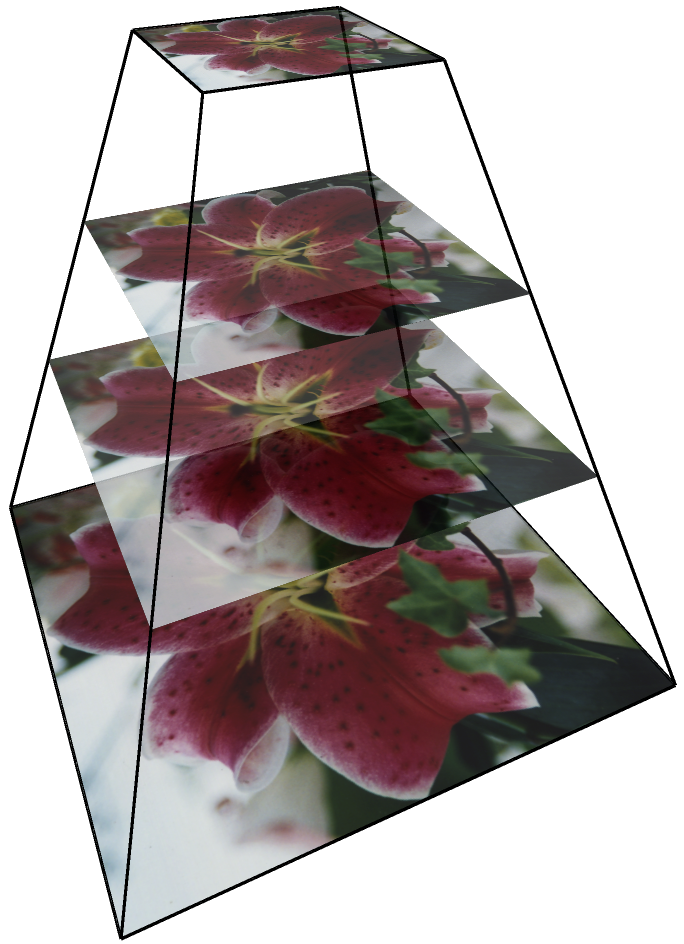
\includegraphics[width=.25\textwidth]{contenu/resources/images/image_pyramid_placeholder}
    \caption[Représentation pyramidale des étages de la pyramide de Gauss]{Représentation en pyramide des étages de la pyramide de Gauss. {\color{red}PLACEHOLDER CREDIT WIKIPEDIA}}
    \label{fig:pyramid-gauss}
\end{figure}

\subsection{Pyramide laplacienne}

La pyramide laplacienne est une autre forme de pyramide, et correspond à un type passe-bande. Comme l'expliquent Burt et Adelson~\cite{burt_laplacian_1983} RE L'intérêt de la pyramide laplacienne réside dans le fait que dans une image, les pixels voisins sont souvent hautement corrélés. Ainsi encoder une image en termes de valeur de pixels n'est pas le plus efficace, puisqu'on a de la redondance d'information. Pour encoder plus efficacement une image, on a besoin d'une représentation plus compacte, et qui décorelle les pixels voisins. La pyramide laplacienne est une méthode qui répond efficacement à ces deux problématiques.

\subsubsection{Construction de la pyramide}

Plutôt que d'encoder la valeur même de chaque pixel, on prédit la valeur que le pixel devrait avoir, et on encode l'erreur de prédiction. La valeur prédite de chaque pixel est obtenue en calculant une moyenne pondérée locale centrée autour du pixel. On crée donc dans un premier temps une image lissée en convoluant l'image avec un filtre correspondant au calcul de la moyenne pondérée. Cette image encode les corrélations locales de l'image, au niveau d'échelle correspondant au filtre choisi, et représente les éléments redondants que l'on cherche à réduire. Pour se faire, on soustrait cette image à l'originale, et on obtient une image exprimant l'erreur de prédiction pour chaque pixel. On a ainsi la relation :

\begin{equation}
    L = I - k * I,
\end{equation}

avec $I$ l'image originale, $L$ l'image d'erreur de prédiction, et $k$ le filtre de moyenne pondérée. Pour la compression d'image, l'intérêt se trouve dans cette ré-écriture, car les pixels de $L$ sont décorrélés et de faible valeur, donc encodables avec peu de bits, et $k*I$ est une image lissée, qui peut être sous-échantillonnée pour obtenir une image de moitié de taille. On n'encode alors que ces deux images, et on obtient ainsi une représentation plus compacte de l'image originale.

On peut répéter ce processus itérativement, en appliquant à chaque fois le même filtre à l'image lissée de résolution inférieure. On enregistre alors seulement les images d'erreur, dont la taille est divisée par 4 à chaque fois, et la dernière image lissée, de taille $N/2^{2d}$, avec $N$ la taille de l'image initiale et $d$ la profondeur désirée. Encore une fois, on peut se représenter cette collection d'images comme une pyramide, en les superposant de la plus grande à la plus petite.

Le filtre de lissage utilisé est un filtre passe-bas, qui moyenne localement l'image, c'est en fait le même genre que l'on utilise pour créer une pyramide gaussienne. En fait, pour construire une pyramide laplacienne, on utilise souvent la pyramide gaussienne de l'image, qui représente toutes les images lissées. On calcule la pyramide gaussienne, puis ensuite la pyramide laplacienne en soustrayant à chaque étage de la pyramide gaussienne l'étage de plus basse résolution, et on obtient ainsi les images d'erreur de prédiction. En se faisant, on fait une légère approximation des images lissées. En effet dans la pyramide gaussienne, il y a une légère perte d'informations entre les étages, puisque l'on supprime des pixels à chaque fois.

Lorsque l'on veut soustraire une image lissée à son image de taille originale, il faut passer par une étape d'expansion. Une méthode communément utilisée pour l'expansion consiste à doubler la taille de l'image, en insérant des zéros entre chaque pixel, puis à appliquer un filtre passe-bas à l'image résultante. On obtient ainsi une image de taille double, qui est une approximation de l'image lissée. On peut alors soustraire cette image à l'image originale, et on obtient l'image d'erreur de prédiction.

\begin{figure}
    \centering
    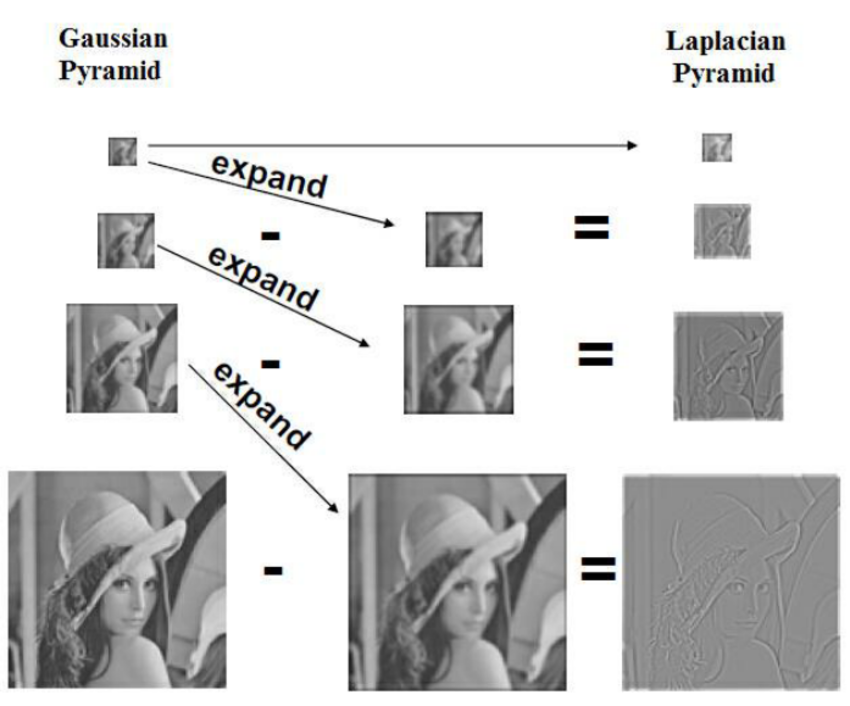
\includegraphics[width=.75\textwidth]{contenu/resources/images/gauss_laplace_pyramid}
    \caption[Relation entre pyramide gaussienne et laplacienne]{Processus de création de la pyramide laplacienne à partir de ma pyramide gaussienne. Image par Jebamalar et Sutha~\cite{jebamalar_design_2014}.}
    \label{fig:gauss-laplace-pyramid}
\end{figure}

\subsubsection{Reconstruction de l'image}

Une fois une image décomposée en pyramide laplacienne, on peut la stocker en enregistrant les images d'erreur de prédiction et l'image lissée de plus basse résolution. Pour reconstruire l'image originale, on procède itérativement. On additionne le résidu basse fréquences, l'image la plus lissée de la pyramide, à la dernière image d'erreur, pour former une image moins lissée. On répète alors le processus, en additionnant à chaque fois l'image lissée obtenue à l'image d'erreur suivante, jusqu'à obtenir l'image originale.

Lorsque l'on utilise une pyramide gaussienne pour créer une pyramide laplacienne, il faut cependant faire attention à la taille des images, qui est divisée par 4 à chaque étage. Pour cela, on étend à chaque étape les images lissées, en utlisant la même opération d'expansion que celle utilisée pour la création de la pyramide. On s'assure ainsi d'opérer sur des images de même taille. Comme à la construction, la reconstruction des images lissées comporte une petite approximation. Puisque l'on travaille avec des images de taille différente, on a perdu de l'information entre les étages. Cependant, à cette étape on additionne les reconstructions d'images lissées, celles qui ont précédemment été soustraites pour la construction. Ainsi, les deux s'annulent, et on a une reconstruction parfaite de notre image originale.

\begin{figure}
    \centering
    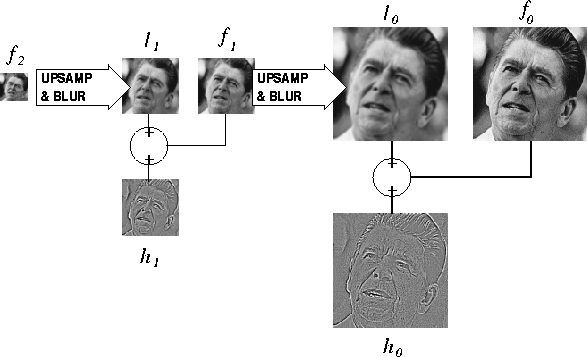
\includegraphics[width=.85\textwidth]{contenu/resources/images/laplacian_pyramid_reconstruction}
    \caption[Reconstruction d'une image à partir de sa pyramide laplacienne]{Reconstruction d'une image à partir de sa pyramide laplacienne. $f_i$ les images de la pyramide gaussienne, $h_i$ celles de la pyramide laplacienne, et $l_i$ les images lissées étendues. Image de \href{https://web.archive.org/web/20230203082428/http://sepwww.stanford.edu/data/media/public/sep/morgan/texturematch/paper_html/node3.html}{Stanford Exploration Project}.}
    \label{fig:laplace-reconstruction}
\end{figure}

\subsection{Pyramide de Riesz}

La pyramide de Riesz est une extension de la pyramide laplacienne. C'est le cadre qui nous permet d'étudier le signal monogène d'une image à différents niveaux d'échelle. On la construit simplement en appliquant la transformée de Riesz à chaque étage de la pyramide laplacienne. On calcule alors les informations locales de chaque étage, que nous mettons ensuite en relation dans nos travaux afin d'extraire plus d'information de notre image.

\begin{figure}
    \centering
    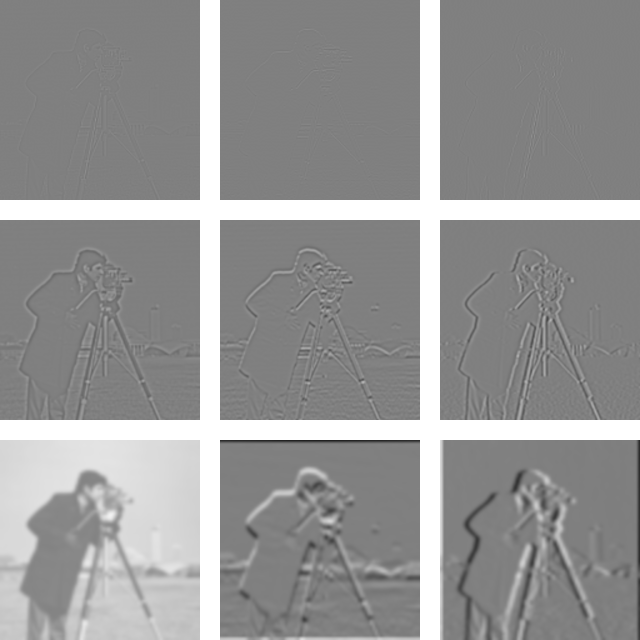
\includegraphics[width=.65\textwidth]{contenu/resources/images/riesz_pyramid_cameraman}
    \caption[Pyramide de Riesz]{Différents étages de notre pyramide de Riesz, calculée avec la transformée de Riesz approximée. En colonne, les différentes composantes : l'image originale de la pyramide laplacienne (gauche), puis les deux composantes de Riesz (milieu et droite). En ligne, les différents étages de la pyramide : étage 0 (haut), étage 2 (milieu) et étage 3, le dernier (bas).}
    \label{fig:riesz-pyramid-cameraman}
\end{figure}

Pour des raisons de vitesse de calcul et de simplicité d'implémentation, nous n'utilisons cependant pas la vraie transformée de Riesz, qui nécessiterait une transformation de l'image dans le domaine de Fourier, ou le calcul d'une intégrale singulière (voir~\ref{eq:riesz-transform-spatial}). À la place, nous reprenons l'approximation utilisée par Wadhwa et al.~\cite{wadhwa_riesz_2014}, qui se calcule directement dans le domaine spatial en utilisant les filtres à réponse impulsionnelle finie $[-0.5, 0, 0.5]$ et $[-0.5, 0, 0.5]^T$, dont les réponses en fréquence sont :

\begin{equation}
    -i\sin(\omega_x) \quad \text{et} \quad -i\sin(\omega_y).
\end{equation}

Cette approximation donne de bons résultats dans notre pyramide, car les filtres ont une réponse équivalente aux alentours de $\frac\pi2$, où se concentre la majorité de l'énergie de nos images dans la pyramide laplacienne~\cite{wadhwa_riesz_2014}. En $0$, la différence notable entre les filtres n'est pas très grave, puisque le contenu fréquentiel est très faible. On rappelle en effet que la pyramide laplacienne est formée en soustrayant à chaque étage une image lissée qui correspond au contenu basse fréquence. Wadhwa et al. proposent une méthode pour calculer une meilleure approximation de la transformée de Riesz à l'aide de filtres finis de plus haut ordre. Nous n'avons cependant pas implémenté cette méthode, car l'approximation basique nous donne déjà de bons résultats. Pour avoir de meilleurs résultats, nous aurions plutôt cherché à implémenter un calcul de la transformée de Riesz passant par le domaine fréquentiel et utilisant la transformée de Fourier.

{\color{red}VOIR TRAVAUX LÉO}


\begin{figure}
    \centering
    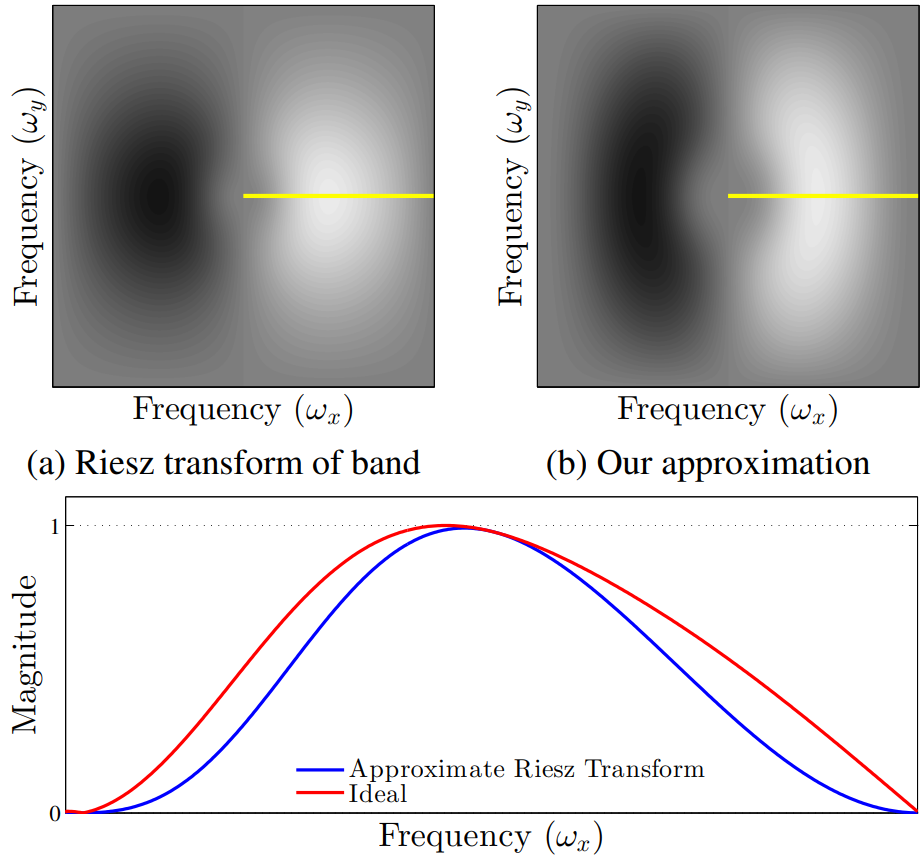
\includegraphics[width=.65\textwidth]{contenu/resources/images/riesz_approximation}
    \caption[Approximation de la transformée de Riesz]{Comparaison de l'application de la transformée de Riesz (gauche) et de son approximation (droite) pour un niveau de pyramide. Les tranches horizontales en jaune sur les images (a) et (b) sont représentés dans le diagramme en (c).}
    \label{fig:riesz-approximation}
\end{figure}

Après avoir fait la transformée de Riesz, on peut calculer pour chaque étage les images d'informations locales, amplitude, phase et orientation.

\begin{figure}[h]
    \centering
    \includegraphics[width=.90\textwidth]{contenu/resources/images/riesz_pyramid_pasta}
    \caption[Informations locales de la pyramide de Riesz]{Informations locales de la pyramide de Riesz. En colonne, les différentes composantes : en colonne, les différentes informations locales : amplitude (gauche), phase (milieu) et orientation (droite). En ligne les différentes étages de la pyramide, du premier (haut) au dernier (bas).}
    \label{fig:riesz-pyramid-local}
\end{figure}

Avec cette implémentation de la pyramide de Riesz, nous avons défini notre cadre d'étude multi-résolutionnel local. Nous allons voir dans la prochaine partie comment nous l'utilisons afin d'extraire de l'information sur nos textures.

\section{Congruence de phase}

Le modèle de l'énergie locale est un modèle de détection de caractéristiques saillantes dans une image. Introduit par Morrone et al~\cite{morrone_mach_1986, morrone_feature_1987},il explique la présence de points saillants, tels que des bords et des coins, par l'alignement des phases locales de l'image. Il est basé sur l'observation que les bords et les coins sont des structures résultant de la superposition de sinusoïdes en phase les unes avec les autres. Contrairement aux autres méthodes de détection de caractéristiques, comme celles de Sobel ou Canny, ce modèle est insensible aux variations de luminosité et de grossissement. Les méthodes par gradient utilisent en effet un seuillage pour déterminer les bords, qui dépend de la luminosité et du niveau de zoom de l'image. À l'inverse, le modèle de l'énergie locale permet le calcul de la congruence de phase, une grandeur à valeurs dans $[0, 1]$ mesurant uniformément la présence de caractéristiques dans une image et, de façon intéressante, la \textit{proximité} à un élément caractéristique. C'est cette grandeur à laquelle nous nous intéressons dans la partie qui suit.

La formulation initiale de la congruence de phase utilise les coefficients de la série de Fourier du signal. Cependant, cette formulation comporte trois problèmes : elle est difficile à calculer et manipuler, elle ne permet pas une bonne localisation de l'information (le même problème qui nous pousse à utiliser un cadre de travail multi-résolutionnel pour l'étude du signal monogène), et RE elle ne prend pas en compte la répartition des fréquences en phase. La solution à ces problèmes se fait par différents moyens, dans un premier temps en 1D, puis en 2D.

\subsubsection{Énergie locale}

Tout d'abord, Venkatesh et Owens~\cite{venkatesh_energy_1989} montrent qu'il existe une relation directe entre la congruence de phase et l'énergie locale. Ils mettent ainsi en lumière une expression simplifiée de la congruence de phase :

\begin{equation}
    PC(x) = \frac{E(x)}{\sum_{n=0}^{+\infty} D_n},
\end{equation}

avec $E(x) = \sqrt{f^2(x) + f_h^2(x)}$ l'énergie locale et $D_n$ les coefficients d'amplitude de la série de Fourier du signal :

\begin{equation}
    f(x) = \sum_{n=0}^{+\infty} D_n\cos(n\omega x + \phi_n).
    \label{eq:phase-congruence-energy}
\end{equation}


\subsubsection{Contexte multi-résolutionnel}

Pour obtenir de l'information localisée en termes de fréquence, Kovesi des ondelettes, sous forme de banque de filtres passe-bande, pour sélectionner successivement différents niveaux d'échelle. Il utilise pour cela des filtres de Gabor, très similaires à ceux présentés dans la section introduisant le signal monogène~\ref{subsubsec:echelle}. En faisant la convolution du signal par ces filtres, il obtient de l'information localisée à la fois spatialement et fréquentiellement :

\begin{equation}
    A_n(x) = \sqrt{(f(x)*M^e_n)^2 + (f(x)*M^o_n)^2},
    \label{eq:local-scale-amplitude}
\end{equation}

et

\begin{equation}
    \phi_n(x) = \arctan\left(\frac{f(x)*M^o_n}{f(x)*M^e_n}\right),
\end{equation}

avec $M^e_n$ et $M^o_n$ les filtres passe-bande, paire et impaire, au niveau d'échelle $n$. À noter que le $n$ dans l'équation~\ref{eq:local-scale-amplitude}, entre 1 et $N$ (le nombre de nivaux d'échelle considéré), désigne le niveau d'échelle fréquentiel. Ce n'est pas le même que celui dans l'équation de la série de Fourier~\ref{eq:phase-congruence-energy} qui, lui, représente les différentes sinusoïdes qui forment le signal. En regardant le scalogramme représenté à la figure~\ref{fig:phase-congruence-scalogram} qui représente l'analyse du signal par la banque de filtres, on voit l'intérêt de la congruence de phase : les points saillants sont ceux où la phase est alignée à travers tous les niveaux d'échelle.

\begin{figure}
    \centering
    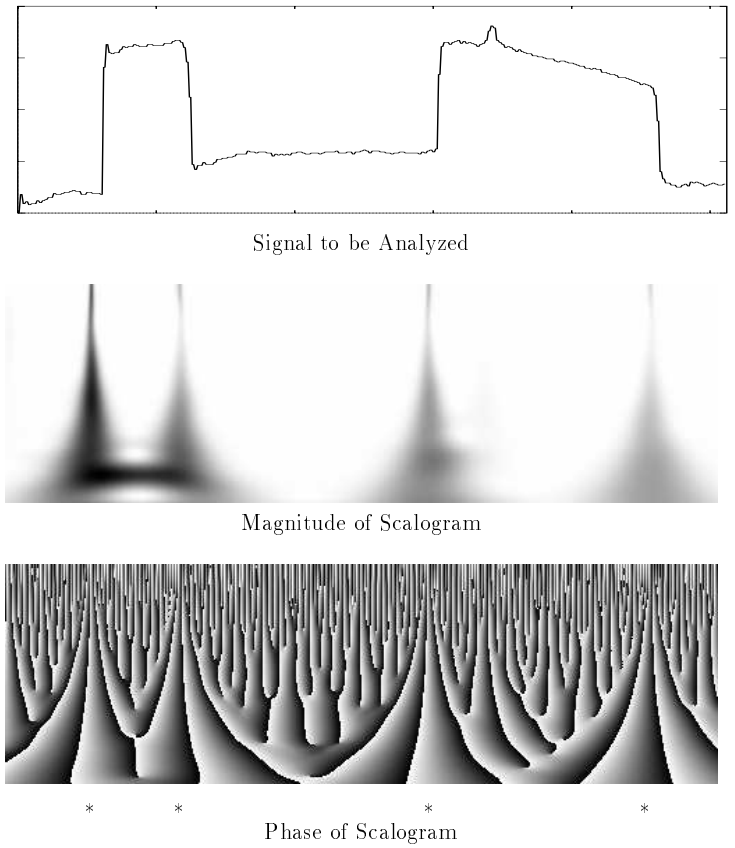
\includegraphics[width=.85\textwidth]{contenu/resources/images/phase_congruence_scalogram}
    \label{fig:phase-congruence-scalogram}
    \caption[Scalogramme d'un signal présentant des points caractéristiques]{Signal 1D et ses scalogrammes de phase et d'amplitude. L'abscisse des scalogrammes sont les mêmes que celui du signal, et les ordonnées représentent à la fréquence en échelle logarithmique (valeurs croissantes de bas en haut). Les astérisques marquent les transitions abruptes dans le signal, et correspondent aux instants où la phase est alignée à travers tous les niveaux d'échelle ; ce sont des points où la congruence de phase est élevée. Image par Kovesi~\cite{kovesi_image_1995}.}
\end{figure}

Avec les composantes filtrées à différents niveaux d'échelle du signal, on obtient une nouvelle expression de la congruence de phase, qui prend en compte la localisation fréquentielle :

\begin{equation}
    PC(x) = \frac{E(x)}{\sum_{n=1}^{N} A_n(x)} = \frac{\sqrt{F^2(x)+F_H^2(x)}}{\epsilon + \sum_{n=1}^{N}},
\end{equation}

avec $F$ et $F_H$ une reconstruction du signal et de sa transformée de Hilbert respectivement, à partir des composantes filtrées :

\begin{align}
    F(x) &= \sum_{n=1}^{N} f(x)*M_n^e, \,\text{et}\\
    F_H(x) &= \sum_{n=1}^{N} f(x)*M{_n^o},
\end{align}

et $\sum_{n=1}^{N} A_n(x)$ la somme des amplitudes locales à tous les niveaux d'échelle :

\begin{equation}
    \sum_{n=1}^{N} A_n(x) = \sum_{n=1}^{N} \sqrt{(f(x)*M^e_n)^2 + (f(x)*M^o_n)^2}
\end{equation}

et $\epsilon$ une petite constante positive qui assure la stabilité numérique de l'expression quand la somme des amplitudes est très petite. Dans notre implémentation, on utilise $\epsilon = 0.01$.

La reconstruction du signal et de sa transformée de Hilbert est possible lorsque l'on choisit avec soin les filtres de la transformée par ondelettes, de telle sorte que leur fonction de transfert se superposent lorsqu'additionnées et recouvrent l'entièreté du spectre du signal, comme montré dans la figure~\ref{fig:wavelet-spectrum-coverage}.

\begin{figure}
           \centering
           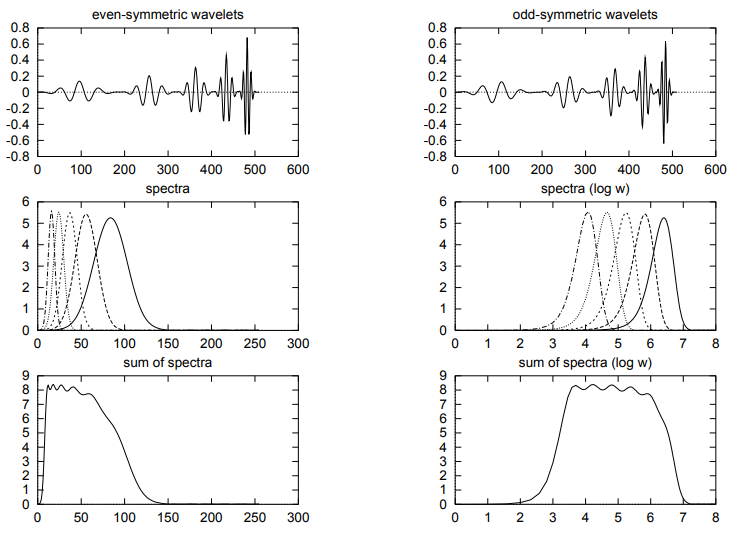
\includegraphics[width=.60\textwidth]{contenu/resources/images/wavelet_spectrum_coverage}
           \caption[Choix des ondelettes pour recouvrir le spectre et permettre la reconstruction du signal]{Banque d'ondelettes choisie de sorte à recouvrir une large couverture du spectre. On voit les ondelettes (haut) et leur fonction de transfert (milieu), et la fonction de transfert de la somme des ondelettes (bas). Image par Kovesi~\cite{kovesi_image_1995}.}
           \label{fig:wavelet-spectrum-coverage}
\end{figure}

\subsubsection{Répartition des fréquences}

La congruence de phase mesure l'alignement des phases à différents niveaux de fréquence, il est donc important qu'une large bande de fréquences soit couverte, afin d'avoir un indicateur significatif. Ceci n'est pas le cas lorsque le signal a une réponse en fréquence restreinte, dans le cas d'un signal simple ou lissé par exemple. La congruence de phase prend alors des valeurs trop grandes sur des plages trop larges du signal, comme montré dans la figure~\ref{fig:phase-congruency-spread}.

\begin{figure}
    \centering
    \begin{subfigure}{.22\textwidth}
        \centering
        
\includegraphics[width=\textwidth]{contenu/resources/images/disk}
        \caption{Image originale\\}
    \end{subfigure}
%    \hfill
    \begin{subfigure}{.22\textwidth}
        \centering
        
\includegraphics[width=\textwidth]{contenu/resources/images/disk_blur}
        \caption{Image lissée}
    \end{subfigure}
    \\
    \begin{subfigure}{.22\textwidth}
        \centering
        
\includegraphics[width=\textwidth]{contenu/resources/images/pc_blur_nospread}
        \caption{Congruence de phase sans pondération}
    \end{subfigure}
%    \hfill
    \begin{subfigure}{.22\textwidth}
        \centering
        
\includegraphics[width=\textwidth]{contenu/resources/images/pc_blur_spread}
        \caption{Congruence de phase avec pondération}
    \end{subfigure}

    \caption{Comparaison de la congruence de phase pour une image lissée par un noyau gaussien, avec et sans pondération par la répartition de la réponse en fréquence.}
    \label{fig:phase-congruency-spread}
\end{figure}

Pour remédier à ce problème, on construit une fonction de pondération qui diminue l'importance des points où la réponse en fréquence est restreinte. On mesure la répartition de la réponse en fréquence en comparant la plus grande amplitude locale à celles des autres niveaux d'échelle :

\begin{equation}
    s(x) = \frac1N\left(\frac{\sum_{n=1}^{N}A_n(x)}{\epsilon + A_{max}(x)}\right),
\end{equation}

où $A_{max}(x)$ la plus grande amplitude parmi ces niveaux et $\epsilon$ est encore une petite constante positive qui assure la stabilité numérique de l'expression. On otient ainsi une mesure de la répartition de la réponse en fréquence à valeurs entre 0 et 1, qui nous permet de construire notre fonction de pondération avec la fonction sigmoïde :

\begin{equation}
    W(x) = \frac{1}{1 + \exp^{g(c-s(x))}},
\end{equation}

avec $c$ la valeur de coupure en-dessous de laquelle on considère que la réponse en fréquence est restreinte, et $g$ un paramètre de gain qui contrôle la précision de la coupure. Dans la pratique, on choisit les valeurs $c = 0.4$ et $g = 10$, qui donne des résultats satisfaisants.

On obtient ainsi une fonction de pondération qui vaut 1 lorsque la réponse en fréquence est uniformément répartie, et qui décroit lorsque la réponse en fréquence est restreinte. On peut alors ré-écrire la congruence de phase en prenant en compte cette fonction de pondération :

\begin{equation}
    PC(x) = \frac{W(x)E(x)}{\epsilon + \sum_{n=1}^{N} A_n(x)}.
\end{equation}

\subsubsection{Extension à deux dimensions}

Pour étendre la méthode en deux dimensions, Kovesi utilise une banque de filtres de Gabor 2D auxquels il applique une fonction d'étalement gaussienne, perpendiculairement à la direction du filtre. En variant l'orientation des filtres, il s'assure de recouvrir totalement le spectre de l'image. L'expression de la congruence de phase s'étend pour prendre en compte toutes les orientations :

\begin{equation}
    PC(\mathbf{x}) = \frac{\sum_{o\in \mathcal{O}} W_o(x)E_o(\mathbf{x})}{\epsilon + \sum_{o \in \mathcal{O}}\sum_{n=1}^{N} A_{no}(\mathbf{x})}
\end{equation},

où $\mathcal{O}$ est l'ensemble des orientations utilisées dans la banque de filtres. Le calcul de la répartition des fréquences $W_o(x)$ doit aussi se faire pour chaque orientation.

\subsubsection{Utilisation du cadre multi-résolutionnel local de Riesz}

Nous souhaitons appliquer le modèle de la congruence de phase pour synthétiser des textures présentant de la structure irrégulière. Cependant, le cadre multi-résolutionnel local de Riesz présenté précédemment nous semble plus intéressant que les banques d'ondelettes de Gabor présentée par Kovesi~\cite{kovesi_image_1995}, car il est plus compacte, plus simple à implémenter, et donne plus d'informations. SY Notamment, il donne accès à l'orientation locale en chaque pixel de l'image, information pertinente pour l'analyse de nos textures. On adapte donc le modèle de la congruence de phase à notre cadre de travail, avec une pyramide de Riesz :

\begin{equation}
    PC(\mathbf{x}) = \frac{W(x)E(\mathbf{x})}{\epsilon + \sum_{n=0}^{d} A_{n}(\mathbf{x})} = \frac{W_(x)\sqrt{F^2(\mathbf{x})+R_1^2(\mathbf{x})+R_2^2(\mathbf{x})}}{\epsilon + \sum_{n=0}^{d} \sqrt{f_n^2(\mathbf{x}) + r_{1n}^2(\mathbf{x}) + r_{2n}^2(\mathbf{x})}},
\end{equation}

avec $d$ la profondeur de la pyramide, $f_i, r_{1i}\, \text{et}\, r_{2i}$ les composantes de Riesz de l'étage $i$, et $F, R_1$ et $R_2$ les reconstructions de l'image originale, et des composantes de sa transformée de Riesz, qui se calculent avec les différents étages de la pyramide :

\begin{equation}
    F(\mathbf{x}) = \sum_{n=0}^{d} f_n(\mathbf{x}) \quad \text{et} \quad R_i(\mathbf{x}) = \sum_{n=0}^{d} r_{in}(\mathbf{x})\, \text{pour}\, i \in \{1, 2\}.
\end{equation}

\begin{figure}
    \centering
    \begin{subfigure}{.3\textwidth}
        \centering
        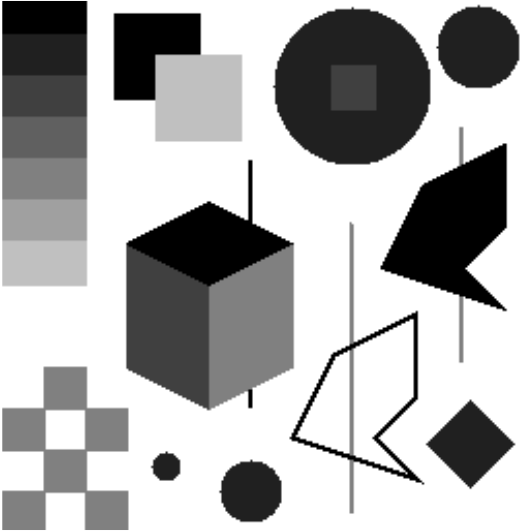
\includegraphics[width=\textwidth]{contenu/resources/images/geometry_shapes}
        \caption{Image originale}
    \end{subfigure}
    \hfill
    \begin{subfigure}{.3\textwidth}
        \centering
        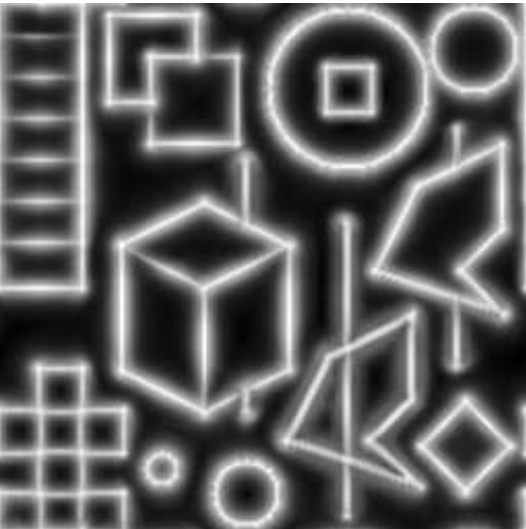
\includegraphics[width=\textwidth]{contenu/resources/images/geometric_shapes_pc_kovesi}
        \caption{Congruence de phase de Kovesi}
    \end{subfigure}
    \hfill
    \begin{subfigure}{.3\textwidth}
        \centering
        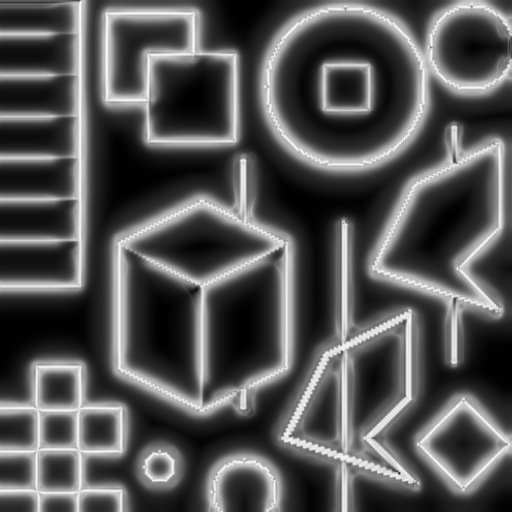
\includegraphics[width=\textwidth]{contenu/resources/images/geometric_shapes_pc_riesz}
        \caption{Congruence de phase de Riesz}
    \end{subfigure}

    \caption{Comparaison de la congruence de phase de Kovesi et de Riesz pour une image de test de formes géométriques.}
    \label{fig:phase-congruency-riesz}
\end{figure}

\bigskip

Avec cette formulation, on a défini une méthode de calcul de la congruence de phase dans notre cadre de travail. Nous allons maintenant voir comment cette méthode a été implémentée, et comment nous l'utilisons pour la synthèse de texture.
